\documentclass{article}

\usepackage[main=english,vietnamese]{babel}
\usepackage[T1]{fontenc}
\usepackage[utf8]{inputenc}
\usepackage[sexy]{evan}
\usepackage{matchsticks}
\usepackage{wrapfig}
\usepackage{listings}

\newtheorem{hint}{Hint}

\title{Counting in two ways}
\author{Nghia Doan}
\date{\today}

\begin{document}

\maketitle

In this article, we show a few example problems that can be solved when using the counting in two ways method.

\begin{example*}[Sum of areas]

    $ABCD$ is a parallelogram. $E$ and $F$ are points on $AB$ and $BC,$ respectively.
    Lines $AF, CE, DE,$ and $DF$ dissect the parallelogram into $8$ regions,
    where some of them have known areas, as shown below in the diagram.

    Find the sum of the areas $a+b+c.$
\end{example*}

\begin{center}
    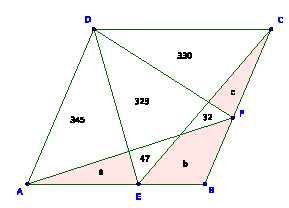
\includegraphics[width=6.5cm]{./svg/pdf/hc-2022-2-2-6.pdf}
\end{center}

\begin{soln}
    From the properties of the parallelogram $ABCD,$ the following triangle pairs, with the same base and height, have the same area
    \[
        \left.
            \begin{aligned}
                [AFB] = [DFB]\\
                [CEB] = [DEB]
            \end{aligned}
        \right\}
        \Rightarrow [AFB] + [CEB] = [DFB] + [DEB] = [DEBF]
    \]

    Therefore
    \[
        (a + 47 + b) + (c + 32 + b) = (323 + 47 + b + 32)
        \Rightarrow a + b + c = \boxed{323.}
    \]
\end{soln}

\begin{example*}[How many knights are needed to protect King Anthony?]

    King Anthony went for hunting trip with his knights.
    At night, they stayed in one of the king's hunting lodges in the forest.
    In this house, there are nine rooms. The king slept in the central room.
    The knights stayed in the eight surrounding rooms such that
    in each direction north, south, east, west the total number of knights 
    in the \textit{three rooms} facing that direction should always be \textit{nine}.
    \textit{For example, the diagram below shows a possible case with each room has 3 knights.
    The letter $K$ indicates the King staying in the central room.}

    \begin{center}
        \begin{minipage}[t]{6.5cm}
            \centering
            \begin{tabular}{|c|c|c|}
                \hline
                $3$ & $3$    & $3$ \\ \hline
                $3$ & K & $3$ \\ \hline
                $3$ & $3$    & $3$ \\ \hline
            \end{tabular}
        \end{minipage}
    \end{center}

    What would be the smallest number of knights were with the king?
    What would be the largest?
\end{example*}

\begin{soln}
    Let $a_1,a_2,a_3,a_4,b_1,b_2,b_3,$ and $b_4$ be the numbers of knights in each room as shown in the diagram.
    Let $S=a_1+a_2+a_3+a_4+b_1+b_2+b_3+b_4,$ then
    \[
        36 = (a_1+b_1+a_2)+(a_2+b_2+a_3)+(a_3+b_4+a_4)+(a_4+b_4+a_1)
        \Rightarrow 
        \begin{cases}
            S = 36 - (a_1+a_2+a_3+a_4)\\
            S = \half\left(36 + (b_1+b_2+b_3+b_4)\right)
        \end{cases}
    \]
    \begin{figure}[h]
        \centering
        \begin{minipage}[t]{6.5cm}
            \centering
            \begin{tabular}{|c|c|c|}
                \hline
                $a_1$ & $b_1$ & $a_2$ \\ \hline
                $b_4$ & K & $b_2$ \\ \hline
                $a_4$ & $b_3$ & $a_3$ \\ \hline
            \end{tabular}
            \caption{With variables}
            \label{fig:hc-2022-1-8-11-2}
        \end{minipage}
    \end{figure}

    Thus, the least value of $S$ is $\boxed{18,}$ if $b_1=b_2=b_3=b_4=0,$ and $a_1=a_3=5,a_2=a_4=4.$
    The most value of $S$ is $\boxed{36,}$ if $a_1=a_2=a_3=a_4=0,$ and $b_1=b_2=b_3=b_4=9.$
\end{soln}

\begin{example*}[What are the family names of the sisters?]

    Four pairs of brother-sister share $32$ cookies.
    For the sisters, Lan got one, Mai got two, Na got three, and Quynh got four cookies.
    Danny Tran took as many as his sister, Elvin Nguyen twice as many as his sister,
    Franklin Pham three times as his sister, and Williams Quach four times as many as his sister.

    What are the family names of the girls?
\end{example*}

\begin{soln}
    
    Let $x, 2y, 3z,$ and $4w$ be the numbers of cookies that 
    Danny Tran, Elvin Nguyen, Franklin Pham, and Williams Quach took.
    Their sisters took $x, y, z,$ and $w$ cookies respectively. Therefore,
    \[
        x + 2y + 3z + 4w + x + y + z + w = 32
        \Rightarrow 2x + 3y + 4z + 5w = 32.
    \]

    Note that $x, y, z, w$ are a permutation of $1,2,3,4,$ so $x + y + z + w = 10.$
    Thus 
    \[
        \begin{aligned}
            &-x + z + 2w = 32-3(x + y + z + w) = 2 \Rightarrow x > z, x \text{\ and\ } z \text{\ have the same parity}\\
            &\Rightarrow -x+z=-2 \Rightarrow  w=2 \Rightarrow x=3, z=1, y=4. 
        \end{aligned}
    \]

    Now, Lan got one, Mai got two, Na got three, and Quynh got four cookies.

    $x=3,$ so the girl who took three cookies, Na, is the sister of Danny Tran, so she is Na Tran.

    $y=4,$ so the girl who took four cookies, Quynh, is the sister of Elvin Nguyen, so she is Quynh Nguyen.
    
    $z=1,$ so the girl who took one cookie, Lan, is the sister of Franklin Pham, so she is Lan Pham.

    $w=2,$ so the girl who took two cookies, Mai, is the sister of Williams Quach, so she is Mai Quach.

    Hence, the girls's names are \framebox{Na Tran, Quynh Nguyen, Lan Pham, and Mai Quach.}
\end{soln}

\end{document}